\chapter{Lo stage}

\section{Aspettative personali}
%\textcolor{OliveGreen}{\textbf{Perchè ho scelto questa azienda e, in particolare, questo progetto di stage e quali erano le aspettative.}}

Non avendo un'esperienza lavorativa nell'ambito dell'informatica, e avendo intrapreso solamente dei progetti didattici nell'ambiente universitario, ho ritenuto necessario scegliere un'azienda per il progetto di \textit{stage}, che riuscisse a far collimare quanto ho studiato nel corso degli anni accademici con quanto viene effettivamente realizzato sul posto di lavoro.
Per scegliere questa azienda ho deciso di partecipare all'iniziativa \textit{"Stage-IT"} organizzata dall'Università di Padova. In questa iniziativa, dedicata all'incontro tra il mondo del lavoro e gli studenti universitari, ho avuto l'occasione di conoscere e di presentarmi a molte aziende, discutendo con loro le varie proposte.
Considerato il grande numero di aziende presenti a questo evento, ho considerato in primo luogo quelle non strettamente legate al mondo dell'informatica e dello sviluppo \textit{software}, quanto piuttosto quelle che utilizzano gli strumenti informatici come ausilio ai sistemi produttivi. In questo modo è possibile vedere sia lo sviluppo che l'applicazione di prodotti software in un ambiente di lavoro, potendo così incrementare le mie conoscenze nel campo dell'\textit{ICT}, della gestione dei processi produttivi e dell'organizzazione aziendale.

Fatte queste considerazioni, ho effettuato dei colloqui conoscitivi con alcune di queste aziende, tra cui \textit{Pietro Fiorentini S.p.A}. Durante questi colloqui l'azienda mi ha presentato diversi progetti, tra i quali ne ho selezionati due:
\begin{itemize}
	\item[•] implementazione di un progetto di \textit{scouting} e di selezione di tecnologie innovative in ambito \textit{ICT}, con lo scopo di applicarle nel miglioramento dei processi aziendali;
	\item[•] progettazione e sviluppo di un'infrastruttura per l'automazione nella creazione di test, con esecuzione e controllo automatizzato dei risultati.
\end{itemize}

Entrambi i progetti mi sono sembrati molto interessanti, in quanto richiedevano un'iterazione con altre figure aziendali. Sebbene il primo potesse sembrare più allettante, vista la completa libertà di ricerca di nuove tecnologie e ambiti di sviluppo, a seguito di un colloquio con il responsabile di tale progetto, ho preferito orientarmi su un'altra tipologia in quanto sembrava poco dettagliato e piuttosto fumoso, e le tempistiche di sviluppo non coincidevano con quanto richiesto dall'Università. Il secondo progetto, invece, mi è sembrato più fattibile e definito, in quanto forniva la possibilità di applicare tutte le tecniche e i meccanismi di test in un contesto reale e pratico.

Durante il colloquio conoscitivo, avvenuto nella sede dell'azienda, ho avuto l'opportunità di conoscere meglio l'azienda stessa e di rivedere e ridefinire alcuni passi della proposta di progetto, anche in relazione alle mie preferenze ed idee. Le aspettative dunque erano tante:
\begin{itemize}
\item[•] entrare in contatto un una grande realtà industriale;
\item[•] conoscere nuove tecnologie;
\item[•] poter lavorare in modo autonomo;
\item[•] realizzare un progetto concreto ed utilizzabile;
\item[•] apprendere i concetti di gestione qualità.
\end{itemize}


\section{Scopo del progetto}
%\textcolor{OliveGreen}{\textbf{Perchè è stato richiesto questo progetto, quali sono le richieste del mercato.}}

%L'attività di progetto proposta da questo \textit{stage} è una continuazione di quanto già proposto ad altri studenti iscritti alla facoltà di informatica dell'Università di Padova.
L'azienda utilizza gli \textit{stage} come mezzo per acquisire nuova forza lavoro da affiancare ai processi produttivi, avendo così la possibilità di percorrere nuove strade senza doversi preoccupare di sacrificarne altre più cruciali. 

La necessità da parte di \textit{Pietro Fiorentini S.p.A} di avviare questo progetto, in continuazione altri simili negli anni precedenti, nasce dalla mancanza nell'organico della divisione \textit{MultiPhase Flow Meter}, di una figura di riferimento con conoscenze specifiche nell'ambito dell'ingegneria del software. É stata richiesta, in particolare, la figura di un amministratore di sistema che fosse in grado di configurare e gestire correttamente gli strumenti di collaborazione e integrazione continua, e che cominciasse ad implementare delle tecnologie per garantire che il \textit{software} prodotto fosse conforme ai processi aziendali, agli standard e alle normative esistenti. 

Il progetto a cui sono stato associato, ha per la prima volta posto l'azienda davanti alla sfida di rilasciare un prodotto software consistente. Tra le richieste dei clienti ricadono specifici standard di qualità e affidabilità, tra cui anche la certificazione CMMI-DEV di livello 2 (Vedi 2.2.1). Da questa particolare richiesta, è nato il desiderio dell'azienda di porre le basi per uno sviluppo controllato e organizzato di tutto il \textit{software} prodotto.


%%%%%%%%%%%%%%%%%%%%%%%%%%%%%%%%%%%%%%%%%%

Questo progetto di \textit{stage} è una continuazione di quanto è stato proposto l'anno scorso ad un altro studente dell'Università di Padova, al quale era stato richiesto di realizzare e implementare degli strumenti per la gestione dei processi come base per la qualità dei prodotti. In quello \textit{stage}, infatti, sono stati implementati degli strumenti di integrazione continua e di collaborazione, ponendo anche delle piccole basi sugli automatismi di analisi statica e dinamica.

A distanza di un anno dallo stage precedente, ho potuto notare che l'azienda crede molto nei risultati ottenuti dagli studenti, infatti, i prodotti di collaborazione e gestione di progetto realizzati, sono entrati a far parte integrante dei processi di sviluppo aziendali.

Dal punto di vista dell'integrazione continua e dell'analisi del codice, sono state solamente poste delle basi per una ingegnerizzazione futura, lasciando molti margini di miglioramento. Non sono state applicate infatti molte regole e metodologie di analisi sul progetto software sviluppato, ma si è preferito studiare e testare, solamente su piccole parti del prodotto, le diverse tecniche per valutare quale fosse la migliore.

La principale attività da me intrapresa, prima di realizzare quanto pianificato dal piano di lavoro, è stata lo studio approfondito di quanto è stato fatto e di quello che si sarebbe potuto ancora fare, basandomi anche sugli sviluppi proposti al termine dello \textit{stage} precedente. Ho riorganizzato poi gli strumenti esistenti, che fino a quel momento erano disorganizzati e salvati su cartelle diverse del \textit{server}, in modo tale da avere una base solida ed ordinata sulla quale lavorare.

%%%%%%%%%%%%%%%%%%%%%%%%%%%%%%%%%%%%%%%%%%


Lo scopo dello \textit{stage} è stato dunque realizzare e utilizzare strumenti di verifica delle metriche interne di qualità del 
\textit{software} (analisi statica, analisi dinamica, etc), revisionando e analizzando in modo automatizzato i risultati, evidenziando le motivazioni e i punti di non conformità. Ho voluto, in accordo con il responsabile, dare una particolare importanza alla documentazione, producendo, per ogni strumento di analisi realizzato, un documento che ne spiegasse le motivazioni e le modalità di utilizzo, e che facesse riferimento ad alcune \textit{best-practice} o normative esistenti. Il progetto della durata di 300 ore, comprendeva quattro fasi principali:
\begin{itemize}
\item[•] Studio dell'esistente e incremento degli strumenti di analisi sullo stile di scrittura del codice;
\item[•] Studio dell'esistente e realizzazione degli strumenti di analisi statica;
\item[•] Realizzazione degli strumenti di analisi dinamica;
\item[•] Realizzazione degli strumenti per la misurazione delle metriche di qualità.
\end{itemize}

I punti chiave richiesti dall'azienda, per ogni fase del progetto, sono stati la realizzazione di una documentazione chiara, necessaria per gestire ed utilizzare gli strumenti, e l'integrazione dei risultati ottenuti con gli strumenti a supporto del progetto realizzati negli \textit{stage} precedenti.

%\section{Punto di partenza}
%\textcolor{OliveGreen}{\textbf{Specifico fino a che punto è arrivato il progetto di stage precedente, e quali sono le nuove aspettative.}}

\subsection{CMMI-DEV 1.3}
\textit{CMMI}, acronimo che sta per \textit{Capability Maturuty Model Integration}, è un modello che fornisce gli strumenti per  per la gestione dei processi. L'obiettivo che si pone, infatti, è guidare la Divisione di Lavoro al miglioramento della gestione dei processi stessi, indicando i punti-chiave che devono sempre essere tenuti in considerazione e ordinandoli secondo livelli di priorità.

Questo modello permette, quindi, di misurare quanto un processo è adeguato per gli scopi per cui è stato definito. Diviso in 5 livelli, il \textit{CMMI} descrive dettagliatamente i processi richiesti per ogni livello e le relative attività, definendone obiettivi e scopi.

Grazie agli \textit{stage} precedenti sono stati coperti e soddisfatti tutti i processi fino al livello 2. Con questo \textit{stage}, invece, si sono voluti stanziare anche i processi di valutazione e validazione appartenenti al livelli 3.

\begin{figure}[H]
  \centering
  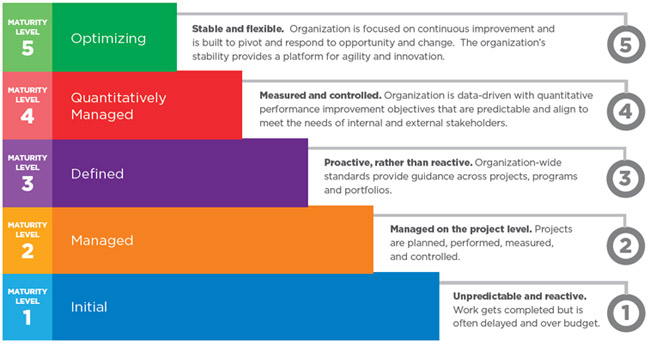
\includegraphics[width=400px]{cmmi.jpg}
  \caption{Livelli e obiettivi CMMI-DEV}
\end{figure}


\section{Obiettivi di progetto}
%\textcolor{OliveGreen}{\textbf{Definisco ciò che è stato richiesto dal piano di Lavoro, dividendo gli obiettivi in minimi e massimi, definendo tempistiche e scadenze settimanali.}}

Alla fine delle 300 ore pianificate dallo \textit{stage}, l'azienda si aspettava un insieme di strumenti funzionanti, almeno su alcuni file sorgenti di prova, per avere una base solida per sviluppi successivi nell'ambito della verifica e validazione del software.
All'inizio dello \textit{stage} ho discusso assieme al \textit{tutor} aziendale gli obiettivi pianificati inseriti all'interno del piano di lavoro, modificando solamente l'ordine temporale di alcuni punti. Gli obiettivi concordati con il \textit{tutor} aziendale sono stati suddivisi in due categorie: minimi e massimi.
\begin{itemize}
\item[•] \textbf{Minimi}
	\begin{itemize}
	\item Aggiunte sezione \textit{"Documentation Plan"} e indicizzazione dei documenti su \textit{Software Quality Plan};
	\item creazione documento \textit{Code style guide} e implementazione di due regole di analisi dello stile di codifica;
	\item creazione documento \textit{Code static analysis} e implementazione di un nuovo controllo di analisi statica;
	\item creazione documento \textit{Software quality metrics} e implementazione con reportistica di una metrica di qualità del software;
	\item creazione documento \textit{Code dynamic analysis} e bozza del piano di test dinamico;
	\item implementazione degli automatismi per un test dinamico;
	\item presentazione di quanto realizzato.
	\end{itemize}
	
\item[•] \textbf{Massimi}
	\begin{itemize}
	\item Completamento sezione \textit{"Measurements"} su \textit{Software Quality Plan};
	\item implementazione completa di 10 regole di analisi dello stile di codifica;
	\item mappatura completa dell'esistente e implementazione di almeno 5 nuovi controlli di analisi statica;
	\item implementazione con reportistica di quattro metriche di qualità del software;
	\item definizione di una \textit{test-suite} con \textit{branch coverage} del 50\%;
	\item implementazione degli automatismi di test dinamici con \textit{branch coverage} del 50\% e completi di reportistica interfacciata con i software di gestione di progetto;
	\item presentazione di quanto realizzato con un \textit{live-demo} interattivo.
	\end{itemize}
\end{itemize}



\section{Vincoli}
%\textcolor{OliveGreen}{\textbf{Specifico le tecnologie già utilizzate all'interno dell'azienda (editor, compilatori, tool esistenti).}}
\subsection{Vincoli metodologici}
Per favorire il dialogo tra studente, \textit{tutor} aziendale e il resto del \textit{team} del reparto di ricerca e sviluppo, lo \textit{stage} si è svolto presso la sede dell'azienda, dandomi così la possibilità di confrontarmi personalmente in caso di dubbi o necessità con i colleghi della divisione, e con il reparto che gestisce i sistemi informativi, in caso di malfunzionamenti del \textit{server}.

Purtroppo non mi è stato possibile confrontarmi con gli sviluppatori \textit{software} in quanto, essendo personale esterno all'azienda, non sono mai stati in sede durante il periodo di \textit{stage}.

Al termine di ogni attività, ho redatto dei documenti ufficiali, in linea con le politiche aziendali, che ricapitolano quanto è stato svolto in modo tale da rendere tracciabile nel miglior modo possibile l'andamento del progetto. Periodicamente, ogni settimana, sono stati effettuati degli incontri con i \textit{tutor} e il responsabile del reparto di Ricerca e Sviluppo, per verificare lo stato di avanzamento, chiarire gli obiettivi ed affinare il piano di lavoro. Al termine del progetto, ho realizzato una presentazione interattiva con i \textit{tutor} aziendali per dimostrare che le attività svolte funzionano e producono i risultati attesi, elencando i pro e contro delle soluzioni trovate, e proponendo eventuali futuri sviluppi.

\subsection{Vincoli temporali}
Lo \textit{stage} pianificato dal \textit{tutor} aziendale, in accordo con l'Università di Padova, ha avuto una durata di 300 ore distribuite nell'arco di otto settimane, dal 02-10-2017 al 24-11-2017. L'orario di lavoro concordato con il reparto Risorse Umane dell'azienda è stato dal Lunedì al Venerdì dalle 7.30 alle 16.30 con un'ora di pausa pranzo.
Il piano di lavoro è stato suddiviso in cinque fasi principali, distribuite nelle otto settimane di lavoro.
\begin{itemize}
\item[•] \textbf{Prima settimana (introduzione)}
	\begin{itemize}
	\item presa visione dell'infrastruttura esistente;
	\item analisi dei requisiti;
	\item stesura documento \textit{"Software Quality Plan"}.
	\end{itemize}
\item[•] \textbf{Seconda settimana (analisi di stile)}
	\begin{itemize}
	\item lettura e aggiornamento documentazione esistente sullo stile di codifica;
	\item aggiornamento \textit{software}  esistente già implementato per il controllo di stile;
	\item verifica automatismi dei report per eventuali non conformità.
	\end{itemize}
\item[•] \textbf{Terza e Quarta settimana (analisi statica)}
	\begin{itemize}
	\item revisione strumenti e \textit{software} di analisi statica esistenti;
	\item definizione e ricerca di nuovi controlli da implementare;
	\item implementazione degli strumenti ricercati e realizzazione della relativa reportistica;
	\item stesura documento \textit{"Code static analysis"}.
	\end{itemize}
	
\item[•] \textbf{Quinta e Sesta settimana (analisi dinamica)}
	\begin{itemize}
	\item definizione e ricerca di nuovi strumenti e di nuove tipologie di test da implementare;
	\item pianificazione e valutazione numero di test necessari a garantire l'adeguata qualità del \textit{software};
	\item implementazione degli strumenti ricercati e realizzazione della relativa reportistica;
	\item esecuzione dei test pianificati.
	\item stesura documento \textit{"Code dynamic analysis"}.
	\end{itemize}

\item[•] \textbf{Settima settimana (metriche di qualità)}
	\begin{itemize}
	\item ricerca e valutazione metriche di qualità;
	\item implementazione delle metriche ricercate e realizzazione della relativa reportistica;
	\item stesura documento \textit{"Software quality metrics"}.
	\end{itemize}

\item[•] \textbf{Ottava settimana (conclusione)}
	\begin{itemize}
		\item incontro per presentare e insegnare ad usare quanto prodotto;
		\item \textit{live-demo} di tutto il lavoro di \textit{stage}

	\end{itemize}
\end{itemize}

\begin{figure}[H]
  \centering
  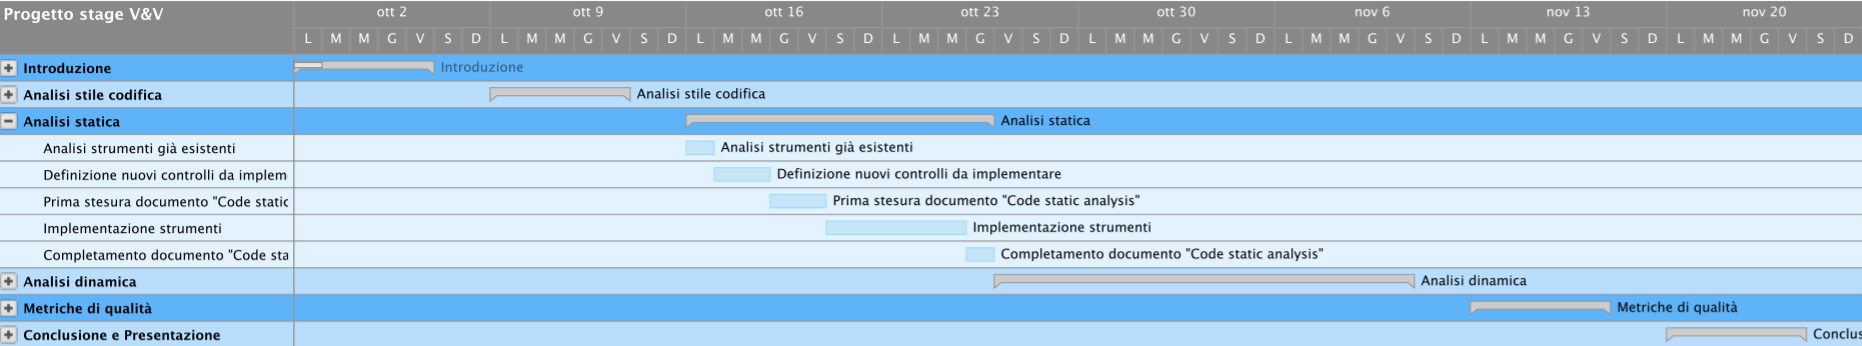
\includegraphics[width=420px]{gantt.png}
  \caption{Diagramma di Gantt con dettaglio attività di analisi statica}
\end{figure}

Rispetto a quanto pianificato inizialmente, il \textit{tutor} ed io abbiamo ritenuto di dover spostare le attività di misurazione delle metriche di qualità dopo la definizione e l'implementazione dei test dinamici, in modo tale da avere una panoramica più precisa su quali metriche applicare, in relazione alla tipologia di test sarebbero stati implementati.

\subsection{Vincoli tecnologici}
L'azienda non ha posto alcun particolare vincolo tecnologico, se non per quanto riguarda l'utilizzo della \textit{suite "IAR System"} per la compilazione ed esecuzione dei codici sorgente da caricare sui misuratori di flusso, e il vincolo di utilizzare prodotti \textit{\glossaryItem{open source}} per quanto riguarda la realizzazione degli strumenti di analisi.

Le scelte tecnologiche da me effettuate sono state vincolate, però, dalle scelte progettuali degli scorsi \textit{stage}, per dare una continuità rispetto quanto è stato prodotto in precedenza. In particolare, per la realizzazione degli \textit{script} automatizzati da far eseguire in modo del tutto indipendente dal \textit{server} e da Jenkins, ho utilizzato il linguaggi \textit{Bash} e \textit{Python}.
La scelta di utilizzare \textit{Bash}, seppure non sia un vero e proprio linguaggio di programmazione, è dettata principalmente sul fatto che il \textit{server} su cui vengono eseguite tutte le tecniche di analisi si basa su una distribuzione \textit{Linux}. I compiti principali che gli strumenti realizzati dovevano svolgere erano principalmente due:
\begin{itemize}
\item eseguire in modo ripetitivo uno o più applicativi di analisi;
\item essere eseguiti in modo automatizzato da altri programmi.
\end{itemize}
Visto l'ambiente di esecuzione e i principali compiti, che ricadono esattamente nelle caratteristiche principali di questo linguaggio, ho ritenuto che fosse quello ideale per raggiungere lo scopo prefissato dallo \textit{stage}. \textit{Python} viene utilizzato per automatizzare i processi in ambiente \textit{Windows Server}. 

Per quanto riguarda la rappresentazione dei risultati dei report di analisi, sono passato dalla visualizzazione su un semplice file di testo, all'integrazione su Redmine, tramite un apposito modulo creato ad-hoc. Le tecnologie utilizzate per creare questo modulo sono state Html e CSS per la rappresentazione grafica. Per la parte dinamica di rielaborazione dei dati storicizzati su un \textit{database} MySql, ho utilizzato invece PHP (tramite apposite API fornite dal sistema) e Javascript. Queste scelte sono state vincolate dall'architettura di Redmine, per permettere la massima integrazione tra i due sistemi.



